\chapter{Turbostratic carbons from ligno-cellulosic biomass}
\label{ch:syntheses}

\newpage

\section{Introduction}

\paragraph{Cigarette Butts}

\paragraph{Porogen impregnation}

\section{Precursor selection, synthesis \& sample designation}
% may need to include more synthetic details depending on methodology section.

The genesis of this synthetic work is linked to results reported in Publication VI, namely the unusually high surface area and microporosity ($ \rm > 4000\ m^2\ g^{-1}$ and $\rm > 90\ \%$ respectively) found for samples derived from the KOH-activation of used cigarette filter derived hydrochar. It was suggested in this report that this porosity was not solely a result of KOH but indeed that other porogens (so-called contaminant-porogens) may be present in the precursor. This made it important to (i) determine the identity of these  contaminant-porogens; (ii) test whether these high levels of (micro-) porosity could be attained using the whole cigarette butt; (iii) ascertain if the removal of these contaminant-porogens had an effect on porosity; and (iv) see if such contaminant-porogens do in fact confer porosity on their own. As a result, samples were synthesised both from public ash trays and from a single brand as well as with and without the wrapping paper. Full synthetic details can be found in table \ref{tb:cb_synthesis}. In all cases, used $\rm 2.5\ g$ cigarette butts (UCBs) were ground in a spice grinder, hydrothermally carbonised with $\rm 25\ cm^3$ water at $250\ ^{\circ}C$ ($\rm 5\ ^{\circ}C\ min^{-1}$), held $\rm 2\ h$ then activated for with or without KOH. After cooling, all samples were washed with HCl for at least $\rm 24\ h$, then filtered and washed with water to give neutral washings. Sample designation is h\textit{A-xTTT}, where \textit{A} is the sample prefix (see table \ref{tb:cb_synthesis}), \textit{x} is KOH:cigarette ratio (wt./wt.), and \textit{TTT} is activation temperature in $^{\circ}C$. A portion of each self activated (i.e. $x = 0$) sample in sets $C$ and $D$ was left unwashed to determine the efficacy of the final washing step. These are indicated with $'$, for example hC-0800$'$ indicates a sample activated at $\rm 800\ ^{\circ}C$ in the absence of activating agent, which was not washed. To refer to the hydrochar itself, the designation is hA-hydrochar, e.g. hydrochar derived from subset h\textit{D} (see table \ref{tb:cb_synthesis}) is hD-hydrochar.

\begin{table}[t]
\caption{Synthetic details of samples derived from cigarette butts.}
\label{tb:cb_synthesis}
\begin{tabularx}{\textwidth}{lXll}
\toprule
\textbf{Prefix} & \textbf{Preparation} & $\mathbf{T\ /\ ^{\circ}C}$ & \textbf{\# Samples} \\ 
\midrule
\textbf{hC}     & From public ash tray; Ash, excess tobacco removed before grinding. Hydrochar washed with $\rm 0.5\ L$ water.              & 600, 700, 800 & 9              \\
\textbf{hD}     &  From public ash tray; Ash, excess tobacco removed before grinding.             & 600, 700, 800 & 9             \\
\textbf{hE}     & Single brand from single smoker. Paper, ash, excess tobacco removed before grinding              & 600, 700, 800 & 3              \\
\bottomrule
\end{tabularx}%
\end{table}

At the same time, these contaminant-porogens ought to be in very close proximity to the cellulose acetate fibers. Their concentration is also relatively low compared to that used in a 'traditional' AC synthesis. As such, the author investigated additional precursors with high amounts of cellulosic material, therein using small amounts of porogen, and mixing the precursor and porogen in such a manner as to both minimise the distance between porogen and precursor, and evenly distribute the porogen. Firstly, sawdust-derived carbons were made by incorporating KOH at weight ratios between 0.00 and 2.00 into the hydrothermal carbonisation step, drying the resultant slurry overnight at $\rm 100\  ^{\circ}C$ and then activating at $\rm 800\ ^{\circ}C$ as usual. Hydrothermal carbonisation occured at 200, 250 or 300 $\rm ^{\circ}C$. These sawdust-derived hydrochars are designated \textit{SAx.xx-HHH} where the prefix \textit{SA} indicates activated sawdust, \textit{x.xx} is the KOH:sawdust ratio and \textit{HHH} is the hydrothermal carbonisation temperature. All samples were washed in the normal manner following activation. The hydrothermally carbonised intermediates are referred to as \textit{SHx.xx-HHH} to differentiate from the activated samples.
% should the lower TTT samples be included?

Additionally, sodium carboxymethyl cellulose (see figure \ref{fig:nc_structure}) was used as a precursor for direct (without hydrothermal carbonisation) activation. The porogen in this case is the sodium carboxymethyl group, and the porogen:precursor ratio is controlled by the degree of substitution. Samples are designated as \textit{NCx.x-TTT} where \textit{NC} indicates sodium carboxymethyl cellulose, \textit{x.x} is the degree of substitution, and \textit{TTT} is the activation temperature. Values for \textit{x.x} were 0.0, 0.7, 0.9, and 1.2 and \textit{TTT} was 600, 700, or 800 $\rm ^{\circ}C$.

\begin{figure}[h]
    \centering
    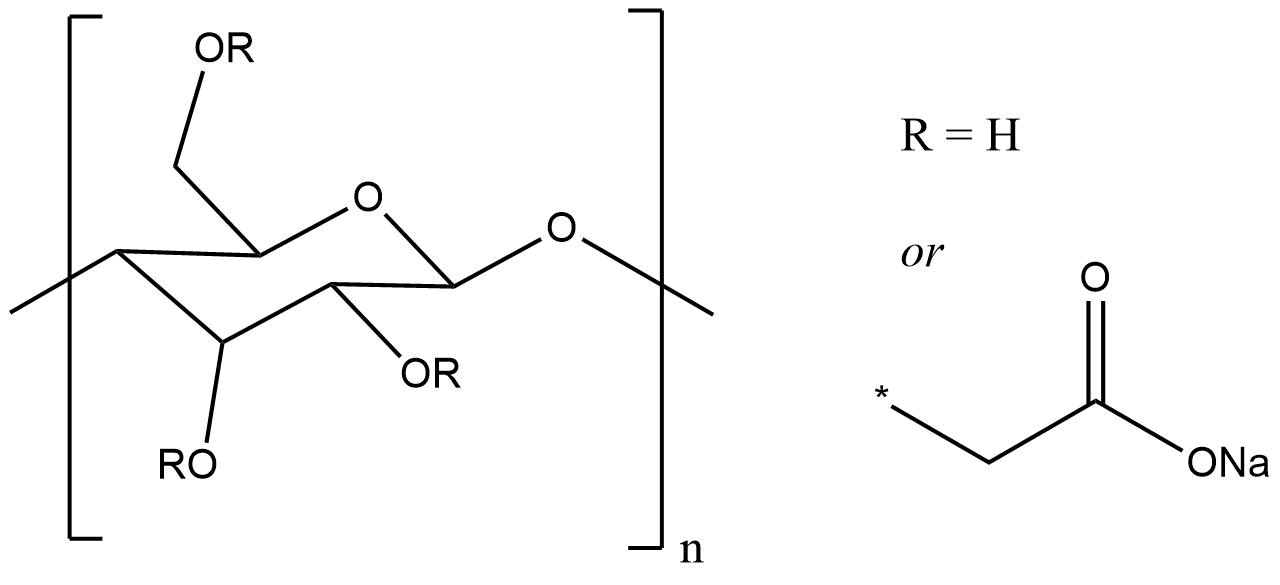
\includegraphics[width=0.8\columnwidth]{4-syntheses/figs/nc_structure.png}
    \caption{Structure of sodium carboxymethyl cellulose. Degree of substitution (DS) is taken as the average number of sodium carboxymethyl groups (\ce{-CH2COONa}) per monomer.}
    \label{fig:nc_structure}
\end{figure}


\section{Results \& Discussion}
\subsection{Cigarette Butts}
\label{ss:cigarette_butts}


\subsubsection{Sample composition}
A primary goal of synthesising the carbons from cigarette butts was quantification and identification of so-called contaminant-porogens in cigarette butts, and monitoring their presence upon conversion of cigarette butts to hydrochar then to turbostratic carbon. Initial identification and rough quantification of the contaminants was performed using P-XRD and TGA respectively, with reference to CHN elemental microanalysis. Attempts were made to identify and more precisely quantify components using XPS and ICP-OES. Finally, imaging of the dispersion of contaminant-metals within unwashed turbostratic carbons was performed using BSE-SEM and EDX-TEM.

\paragraph{Cigarette Butts}

\paragraph{Hydrochars}
In the case of samples in sets \textit{hC} and \textit{hD} 

\paragraph{Activated Carbons}

\subsubsection{Porosity}

\subsubsection{\ce{CO2} uptake}

\subsection{Sawdust}
\label{ss:sawdust}

\subsection{Sodium Carboxymethyl Cellulose}
\label{ss:nc}

\subsubsection{Composition}

\subsubsection{Porosity}

\paragraph{Hysteresis}

\subsubsection{\ce{CO2} uptake}

\section{Conclusions}

\bibliographystyle{rsc}
\bibliography{bibliography/bib}

\section*{Appendix}